%%%%%%%%%%%%%%%%%%%%%%%%%%%%%%%%%%%%%%%%%%%%%%%%%%%%%%%%%%%%%%%
%
% Welcome to Overleaf --- just edit your LaTeX on the left,
% and we'll compile it for you on the right. If you open the
% 'Share' menu, you can invite other users to edit at the same
% time. See www.overleaf.com/learn for more info. Enjoy!
%
%%%%%%%%%%%%%%%%%%%%%%%%%%%%%%%%%%%%%%%%%%%%%%%%%%%%%%%%%%%%%%%
\documentclass{beamer}

\usefonttheme{professionalfonts}
\mode<presentation> {
\usetheme{default}
\usecolortheme{seahorse}
}
\usepackage{ulem}
\usepackage{algorithm2e,algorithmic}
\usepackage{url,amsmath, tikz-cd}
\usepackage{graphicx} % Allows including images
\usepackage{booktabs} % Allows the use of \toprule, \midrule and \bottomrule in tables
\usepackage{mathtools}


\newcommand{\NN}{\mathbb{N}} % Natural numbers
\newcommand{\ZZ}{\mathbb{Z}} % Integers
\newcommand{\QQ}{\mathbb{Q}} % Rationals
\newcommand{\RR}{\mathbb{R}} % Real numbers
\newcommand{\CC}{\mathbb{C}} % Complex numbers
\newcommand{\FF}{\mathbb{F}} % Finite field
\newcommand{\PP}{\mathbb{P}} % Projective space
\newcommand{\Spec}{\text{Spec}} %Spec
\newcommand{\Max}{\text{Max}} %MaxSpec
\newcommand{\HH}{\mathbb{H}}


\newtheorem{proposition}{Proposition}
\newtheorem{remark}{Remark}
\newtheorem{question}{Question}
\BeforeBeginEnvironment{question}{
  \setbeamercolor{block title}{use=example text,fg=white,bg=example text.fg!75!black}
  \setbeamercolor{block body}{parent=normal text,use=block title example,bg=block title example.bg!10!bg}
}
\AfterEndEnvironment{question}{
  \setbeamercolor{block title}{use=structure,fg=white,bg=structure.fg!75!black}
  \setbeamercolor{block body}{parent=normal text,use=block title,bg=block title.bg!10!bg}
}
\newtheorem{answer}{Answer}
\newtheorem{hypothesis}{Hypothesis}
\newtheorem{conjecture}{Conjecture}
\BeforeBeginEnvironment{conjecture}{
  \setbeamercolor{block title}{use=alerted text,fg=white,bg=alerted text.fg!75!black}
  \setbeamercolor{block body}{parent=normal text,use=block title alerted,bg=block title alerted.bg!10!bg}
}
\AfterEndEnvironment{conjecture}{
  \setbeamercolor{block title}{use=structure,fg=white,bg=structure.fg!75!black}
  \setbeamercolor{block body}{parent=normal text,use=block title,bg=block title.bg!10!bg}
}
\newtheorem{metaconjecture}{Meta-Conjecture}
\newtheorem{philosophy}{Philosophy}
\newtheorem{claim}{Claim}
\newtheorem{exercise}{Exercise}

\newtheorem{warning}{Warning}
\BeforeBeginEnvironment{warning}{
  \setbeamercolor{block title}{use=alerted text,fg=white,bg=alerted text.fg!75!black}
  \setbeamercolor{block body}{parent=normal text,use=block title alerted,bg=block title alerted.bg!10!bg}
}
\AfterEndEnvironment{warning}{
  \setbeamercolor{block title}{use=structure,fg=white,bg=structure.fg!75!black}
  \setbeamercolor{block body}{parent=normal text,use=block title,bg=block title.bg!10!bg}
  
}

\DeclareMathOperator{\coker}{coker}
\DeclareMathOperator{\End}{End}
\DeclareMathOperator{\Ext}{Ext}
\DeclareMathOperator{\GL}{GL}
\DeclareMathOperator{\SL}{SL}
\DeclareMathOperator{\Gal}{Gal}
\DeclareMathOperator{\Gr}{Gr}
\DeclareMathOperator{\Hom}{Hom}
\DeclareMathOperator{\OG}{OG}
\DeclareMathOperator{\PGL}{PGL}
\DeclareMathOperator{\Proj}{Proj}
\DeclareMathOperator{\PSL}{PSL}
\DeclareMathOperator{\SO}{SO}
\DeclareMathOperator{\SpG}{SpG}
\DeclareMathOperator{\Stab}{Stab}
\DeclareMathOperator{\Sym}{Sym}
\DeclareMathOperator{\Trace}{Trace}
% \DeclareMathOperator{\det}{det}
\DeclareMathOperator{\Div}{Div}



\renewcommand{\footnotesize}{\fontsize{5pt}{7}\selectfont}



\title{$p$-adic Integration on Modular Curves and Code-based Cryptography}
\author{Jun Bo Lau}
\institute{UCSD}
\date{31 May 2023}

\begin{document}

\frame{\titlepage}

\begin{frame}
\frametitle{Overview} % Table of contents slide, comment this block out to remove it
\tableofcontents % Throughout your presentation, if you choose to use \section{} and \subsection{} commands, these will automatically be printed on this slide as an overview of your presentation
\end{frame}


%----------------------------------------------------------------------------------------
%	PRESENTATION SLIDES
%----------------------------------------------------------------------------------------

\chapter{Preliminaries}

All curves in this paper are smooth, projective and geometrically irreducible with good reduction at a prime $p$.

\section{Introduction}

Some of the oldest questions in number theory can be reformulated in modern terms: given a finite list of polynomials, what are the integer or rational solutions to this set of equations? In fact, these solutions can be viewed as integer or rational solutions of geometric objects -- curves, surfaces or higher dimensional objects.

In this project, we focus on the case of curves. A remarkable result, formulated by Mordell in 1922 and proved by Faltings in 1983, states that for curves of higher genus, there are only finitely many rational points on them. 

\begin{theorem}{(Mordell's conjecture/ Faltings's theorem)} Let $X/\QQ$ be a curve of genus $g \geq 2$, then the set of rational points $X(\QQ)$ is finite.
\end{theorem}

However, Faltings's proofs are not effective, i.e., there is no way of explicitly determining the complete set of rational points on the curve. Before Faltings, Chabauty developed a method in this direction with the condition that if the rank of the Jacobian of the curve is strictly less than the genus, then one could compute this set of points. In \cite{Coleman2,Coleman3} Coleman defined $p$-adic line integrals and re-interpreted Chabauty's method to explicitly compute the set of rational points. These Coleman integrals provide an effective method to problems in arithmetic geometry, including but not limited to, torsion points on Jacobians of curves ( Manin-Mumford conjecture), $p$-adic heights on curves, $p$-adic polylogarithms, Mordell conjecture (rational points), etc. In \cite{BD1,BD2}, Balakrishnan and Dogra developed quadratic Chabauty as a computational tool to study the set of rational points as long as the curve satisfies a certain quadratic Chabauty bound, involving the rank of the Jacobian, genus and N\'{e}ron-Severi rank of the Jacobian.

There are several approaches to numerically compute these Coleman integrals. Wetherell \cite{wetherell} combined the certan properties of Coleman integrals and the arithmetic of the Jacobian to compute $\int_D \omega$, where $D$ is a divisor in the Picard group and $\omega$ is a holomorphic differential on the curve. The next approach relies on computing the Frobenius action in $p$-adic cohomology following Dwork's principle of analytic continuation along the Frobenius \cite{BBK10,Tui16,Tui17,BT_coleman}. However, both of these approaches have their shortcomings -- Wetherell's method requires an explicit divisor in order to reduce the computation to a power series integration (``tiny integrals") and the second method requires an explicit equation of the curves as input.

We turn our attention to computing Coleman integrals on modular curves. The set of rational points on modular curves has special arithmetic meaning. For instance, the set of rational points $X_0(N)(\QQ)$ correspond to the torsion points of elliptic curves (Mazur's theorem). Another motivation to study modular curves comes from Serre's Uniformity Conjecture. Let $E$ be an elliptic curve defined over $K$. The group of $p$-torsion points $E[p](\bar{K})$ is isomorphic to $(\ZZ/p\ZZ)^2$ and is acted upon by the absolute Galois group $\Gal(\bar{K}/K)$, giving rise to a representation $\rho_ {p,E}: \Gal(\bar{K}/K) \rightarrow \GL_2(\FF_p)$. In \cite{serre72}, Serre proved the following:

\begin{theorem}
    Suppose that $E$ does not have complex multiplication. Then there exists a number $N(E)$ such that $\rho_{p,E}$ is surjective for all $p > N(E)$.
\end{theorem}

In the same paper, he posed the following question:

\begin{conj}{(Serre's Uniformity Conjecture)}
Given a number field $K$, then there exist a constant $N_K>0$ such that for any elliptic curve $E$ defined over $K$ without complex multiplication, the corresponding Galois representation $\rho_{p,E}$ is surjective for all primes $p > N_K$.
\end{conj}

Since modular curves parametrise elliptic curves with torsion data, this can be formulated in terms of rational points on modular curves:

\begin{conj}{(Serre's Uniformity Conjecture)}
    Let $H \leq \GL_2(\FF_p)$ be a proper subgroup such that the determinant map $\det: H \rightarrow \FF_p^\times$ is surjective, then there exist a constant $N_K>0$ such that for any prime $p> N_K$, the associated modular curve $X_H(p)$ has $K$-rational points coming only from cusps and elliptic curves with complex multiplication.
\end{conj}




If $\rho_{p,E}$ is not surjective, the image lies inside some maximal proper subgroup of $\GL_2(\FF_p)$. Therefore, one could prove the conjecture by showing that for $p$ large enough, the image of $\rho_{p,E}$ does not lie in any maximal subgroup. The classification of maximal subgroups of $\GL_2(\FF_p)$ is known, originally due to \cite{dickson}:

\begin{theorem}
    Let $H \leq \GL_2(\ZZ/p\ZZ)$ not containing $\SL_2(\ZZ/p\ZZ)$. Up to conjugacy, $H$ is one of the following:
    \begin{itemize}
        \item (Borel) $H \subseteq B_0(p) = \{ \begin{psmallmatrix} \ast \ \ast \\ 0 \ \ast \end{psmallmatrix} \}$ 
        \item (Normaliser of split Cartan) $H \subseteq N_s^+(p) = \{ \begin{psmallmatrix} \alpha \ 0 \\ 0 \ \beta \end{psmallmatrix}, \begin{psmallmatrix} 0 \ \alpha \\ \beta \ 0 \end{psmallmatrix}: \alpha,\beta \in \FF_p^\times \}$ 
        \item (Normaliser of non-split Cartan) $H \subseteq N_s^+(p) = \{ \begin{psmallmatrix} \alpha \ 0 \\ 0 \ \alpha^p \end{psmallmatrix}, \begin{psmallmatrix} 0 \ \alpha \\ \alpha^p \ 0 \end{psmallmatrix}: \alpha \in \FF_{p^2}^\times \}$ 
        \item (Exceptional) The image of $H$ in $\PGL_2(\FF_p)$ is isomorphic to $A_4,S_4$ or $A_5$.
    \end{itemize}
\end{theorem}

Most of the cases have been resolved \cite{borel,BP1,BP2,serre72}, except for the normaliser of non-split Cartan. There has been some progress using quadratic Chabauty to find the rational points of the modular curve corresponding to the nonsplit Cartan of level 13 \cite{cursed-curve} and level 17 \cite{BDMTV}.

Since most modular curves satisfy the quadratic Chabauty bound \cite{Siksek}, we provide a model-free algorithm to compute Coleman integrals on modular curves arising  arising from Serre's Uniformity Conjecture.

\subsection{Modular curves and Hecke operators}

\begin{frame}{Contributions (joint work with Chen-Kedlaya)}
\begin{itemize}
\item We develop an algorithm that computes Coleman integrals on modular curves.
\item The algorithm does not rely on models.
\item We compute some examples of well-known modular curves.
\end{itemize}
\end{frame}

\begin{frame}{Modular curves}
Let $\Gamma \leq \SL_2(\ZZ)$ be a congruence subgroup. The (compactified) quotient space $X(\Gamma) := \Gamma \backslash (\HH \cup \PP^1(\QQ))$ is called the \textit{modular curve with level $\Gamma$}.

\begin{itemize}
\item Riemann surfaces (genus/ramification theory, Riemann-Hurwitz, Riemann-Roch, etc.)
\item Algebraic curves (curves-fields correspondence)
\item Moduli spaces of elliptic curves with torsion
\end{itemize}

\end{frame}

\begin{frame}{Hecke operators}
Let $\Gamma_1,\Gamma_2 \leq \SL_2(\ZZ)$ be congruence subgroups and $\alpha \in \GL_2^+(\QQ)$. We define the double coset $\Gamma_1 \alpha \Gamma_2$ as the set

\[
\Gamma_1 \alpha \Gamma_2 := \{ \gamma_1 \alpha \gamma_2: \gamma_1 \in \Gamma_1, \gamma_2 \in \Gamma_2 \}
\]

These sets give rise to \textit{double coset operators} which act on both the $1$-forms and the points on the modular curves.

\end{frame}

\begin{frame}{Hecke operators on $1$-forms}

For a congruence subgroup $\Gamma$, we have an isomorphism between the space of holomorphic $1$-forms on $X(\Gamma)$ and the space of weight $2$ cusp forms of level $\Gamma$. For $\alpha \in \GL_2^+(\QQ)$, we define the double coset operator:

\[
f|_2 [\Gamma_1 \alpha \Gamma_2] = \sum_i f|_2 \beta_i
\]

where $f$ is a weight $2$ cusp form of level $\Gamma_1$, $\Gamma_1 \alpha \Gamma_2 = \cup_i \Gamma_1 \beta_i$. Hecke operators at $p$ are double coset operators when $\Gamma_1= \Gamma_2 = \Gamma$ and $\det(\alpha) = p$.

\end{frame}

\begin{frame}{Hecke operators on points}

For $\Gamma_1, \Gamma_2$ congruence subgroups, $\alpha \in GL_2^+(\QQ) $, define $\Gamma_3 := \alpha^{-1} \Gamma_1 \alpha \cap \Gamma_2$ and $\Gamma_3' := \alpha \Gamma_3 \alpha^{-1}$. We have a diagram at the level of groups and the corresponding modular curves:

\begin{align*}
\Gamma_2 \hookleftarrow \Gamma_3 \xrightarrow{\cong} \Gamma_3' \hookrightarrow \Gamma_1 \\
X_2 \xleftarrow{\pi_2} X_3 \xrightarrow{\cong} X_3' \xrightarrow{\pi_1} X_1
\end{align*}

Suppose $\Gamma_3 / \Gamma_2 = \bigcup_j \Gamma_3 \gamma_{2,j}$ and $\beta_j = \alpha \gamma_{2,j}$. Then the double coset operator induces a map on the divisor groups:

\begin{align*}
    \Div(X_2) &\rightarrow \Div(X_1) \\
    \Gamma_2 \tau &\mapsto \sum_j \Gamma_1 \beta_j \tau
\end{align*}

\end{frame}

\begin{frame}{Hecke operators on points}

Consider fiber product $X(\Gamma, p) := X_0(p) \times_{X(1)} X(\Gamma)$. There are two degeneracy maps $\alpha,\beta: X_H(p) \rightarrow X_H$ defining the Hecke operator at $p$ where one forgets the cyclic group of order $p$ and the other quotients out by the cyclic group of order $p$.

\[
X(\Gamma) \xleftarrow{\alpha} X(\Gamma,p) \xrightarrow{\beta} X(\Gamma)
\]

This gives an algebraic description of the Hecke operator at $p$:
\[
T_p(E,\mathfrak{n)} := \alpha^* \beta_* (E,\mathfrak{n}) = \sum_{f:E\rightarrow E', deg(f) = p} (E',f(\mathfrak{n})).
\]

\end{frame}


\subsection{Coleman integration on modular curves}

\begin{frame}{Coleman integration on modular curves}

For a congruence subgroup $\Gamma$ and two points $P,Q \in X(\Gamma)$, we compute $\int_P^Q \omega$ in the following way:

\begin{enumerate}
\item (Reduction step) Write any arbitrary Coleman integral as a sum of tiny integrals,
\item (Basis and uniformiser) Find a basis of holomorphic $1$-forms and a suitable uniformiser,
\item (Hecke action) Compute the action of Hecke operator on differential forms and points,
\item (Linear algebra over $\mathbb{C}$) Solve a system of equations and recover algebraic solutions,
\item (Evaluation) Formally integrate and evaluate the end points.
\end{enumerate}
\end{frame}

\begin{frame}{(Reduction) Fundamental system of equations}
Let $\Gamma$ be a congruence subgroup, $\omega_i \in H^0(X(\Gamma), \Omega^1)$, $P,Q \in X(\QQ_p)$, $p >2$ a prime of good reduction. We have:

\[
\int_Q^R T_p^* \omega_i = \sum_j \int_Q^R A_{ij} \omega_j = \sum_j \sum_k \int_{Q_k}^{R_k} \omega_j.
\]

where $T_p Q = \sum_k Q_k.$ This gives the following system of equations: 

\begin{equation*}
   ((p+1)I-A)\begin{pmatrix} \int^Q_R\omega_1 \\\vdots \\ \int^Q_R\omega_g \end{pmatrix} =  \begin{pmatrix} \sum_{i=0}^{p}\int^Q_{Q_i} \omega_1 - \sum_{i=0}^{p}\int^R_{R_i} \omega_1 \\\vdots \\ \sum_{i=0}^{p}\int^Q_{Q_i} \omega_g - \sum_{i=0}^{p}\int^R_{R_i} \omega_g \end{pmatrix}.
\end{equation*}

\end{frame}

\begin{frame}{Next steps}

\begin{equation*}
   ((p+1)I-\textcolor{red}{A})\begin{pmatrix} \int^Q_R\omega_1 \\\vdots \\ \int^Q_R\omega_g \end{pmatrix} =  \begin{pmatrix} \textcolor{blue}{\sum_{i=0}^{p}\int^Q_{Q_i} \omega_1 - \sum_{i=0}^{p}\int^R_{R_i} \omega_1} \\\vdots \\ \textcolor{blue}{\sum_{i=0}^{p}\int^Q_{Q_i} \omega_g - \sum_{i=0}^{p}\int^R_{R_i} \omega_g} \end{pmatrix}.
\end{equation*}

\begin{itemize}
\item \textcolor{red}{Action of Hecke operator at $p$ on basis of cusp forms},
\item \textcolor{blue}{Sums of tiny integrals},
\begin{itemize}
\item Action of Hecke operator on points,
\item Basis of cusp forms in terms of uniformiser
\end{itemize}
\end{itemize}

\end{frame}

\begin{frame}{Action of Hecke operator on cusp forms}

For the congruence subgroups $\Gamma_H$ induced by $H \leq \GL_2(\ZZ/N\ZZ)$, $H^0(X(\Gamma_H),\Omega^1) \cong S_2(\Gamma(N))^H$. A modification of Zywina's Magma implementation \footnote{D. Zywina, \href{https://arxiv.org/abs/2001.07270}{Computing actions on cusp forms}} allows us to compute a basis of $H^0(X(\Gamma_H),\Omega^1)$.

Then, using the double coset definition of Hecke operators, one expresses $f|_2 [\Gamma_H \alpha \Gamma_H]$ as a linear combination of basis elements.
\end{frame}

\begin{frame}{Computing $\sum_i \int_{Q_i}^Q \omega $}
\begin{enumerate}
\item Pick a uniformiser $u$ and write $\omega = \sum_j x_j u^j du$,
\item Calculate $u(Q_i)$ as algebraic numbers,
\item Evaluate $\sum_i \int_{Q_i}^Q \omega = \sum_i \int_{u(Q_i)}^{u(Q)} \omega(u) du$.
\end{enumerate}
\end{frame}

\begin{frame}{Examples}

The algorithm works for:

\begin{itemize}
\item Modular curves coming from maximal proper subgroups of $\GL_2(\ZZ/N\ZZ)$ (Serre's Uniformity Conjecture),
\item Modular curves quotiented by the action of Atkin-Lehner involutions.
\end{itemize}

Each example has its input data:

\begin{itemize}
\item Uniformisers,
\item Basis of cusp forms,
\item Known rational points,
\item Hecke action.
\end{itemize}
\end{frame}
\chapter{Preliminaries}


\section{Introduction}
Most cryptosystems implemented today rely on certain hard problems in number theory, such as factorisation or the discrete log problem. These problems fall into the general category of Hidden Subgroup Problems. Recently, there has been significant research on quantum computers and quantum algorithms which make use of quantum phenomena to solve some of these problems that are deemed difficult on classical computers(\cite{Shor,Jozsa}). 

While building a large-scale quantum computer is an engineering challenge, some scientists predict that within the twenty to fifty years, sufficiently powerful quantum computers will be built to break most if not all current public key cryptography infrastructure. Taking into account the amount of time to implement quantum resistant cryptosystems in public, the National Institute of Standards and Technology (NIST) initiated a process in 2016 to standardise post-quantum digital signature algorithms (DSA), public-key encryption (PKE), and key-encapsulation mechanisms (KEM). Initially, there were 82 submissions. As of April 2023, there 4 algorithms are selected for standardisation while there are three code-based candidates that are still going through evaluation. There is also an on-ramp call for new DSA's in order to diversify the signature portfolio to include signature schemes that are not based on lattices.

\begin{table}[]
\centering
\begin{tabular}{lll}
\hline
 & PKE/KEM & DSA \\ \hline
Selected &  &  \\ \hline
Lattice & 1 & 2 \\
Hash & 0 & 1 \\ \hline
Candidates &  &  \\ \hline
Code & 3 & 0 \\ \hline
\end{tabular}
\caption{NIST Post-Quantum Standardisation Process - Round 4}
\end{table}

In this document, we focus on code-based cryptography, more specifically, one of the 4th round candidates in NIST's standardisation process, BIt-flipping Key Encapsulation (BIKE) \cite{BIKE}. In 1978, McEliece introduced the use of error-correcting codes in cryptography \cite{mceliece}. Originally, error-correcting codes are used in telecommunications in which one party transmits a message through a noisy channel and the recipient recovers the original message from a noisy codeword. In McEliece's proposal, one would use a structured code and hide a message by adding as many errors as the decoder can remove so that the codewords are indistinguishable from random codes. So far, there are no major classical or quantum attacks on the McEliece system but the downside is that it suffers from having large key sizes which make implementations costly.

BIKE is an instance of a more general scheme, called Quasi-Circulant Moderate Density Parity Check (QC-MDPC) codes \cite{QCMDPC}. QC-MDPC codes have much smaller key sizes compared to the McEliece cryptosystem and have not suffered from major attacks. One difference between QC-MDPC codes and McEliece's variants is that QC-MDPC codes use decoders which depend on probabilitistic properties, not algebraic ones. Therefore, one expects decoding failures to occur. Furthermore, decoding failures also reveal information about the secret key. An attack by \cite{GJS} exploits these failures by collecting a set of failure-causing inputs and recover the secret key. With this in mind, one needs to consider the use of ephemeral versus statis keys in applications and also verify certain security conditions, called indistinguishability under chosen cipher attack (IND-CCA). NIST has considered BIKE as one of the promising candidates and has expressed concerns about its IND-CCA security and decoding failure analysis. 

By design, it is not feasible to directly compute the average Decoding Failure Rate (DFR) for BIKE at cryptographic security levels. It is possible to measure DFR's via extrapolation methods to estimate the DFR for larger parameters from smaller ones \cite{SV:2019:extrapolate,DGK20a}. But one needs to consider a phenomenon known as the \textit{error floor} region of DFR curves to avoid an underestimate of DFR for larger code sizes.  It is known that for LDPC and MDPC codes, the logarithm of the DFR drops significantly faster than linearly, and then linearly as the signal-to-noise ratio is increased \cite{bgf,Richardson03}. Thus a typical DFR curve contains a concave \textit{waterfall} region followed by a near-linear \textit{error floor} region. One must accurately predict the error floor of a DFR curve to accurately predict the DFR for cryptographically relevant code sizes.

For LDPC codes, the error floor regions have been studied extesively via their Tanner graph representations. Recent work \cite{Vasseur-thesis,Vasseur:2021:eprint} has considered several factors affecting the DFR of QC-MPDC codes: choice of decoder \cite{tillich:2018:decoding,SV:2019:extrapolate}, classes of weak keys, and sets of problematic error patterns.

Our approach to this problem is to study a scaled-down version of BIKE, and identify various properties of QC-MDPC codes and their decoding failures through extensive experiements.
\subsection{BIKE and QC-MDPC codes}

\begin{frame}{Binary linear codes and QC-MDPC codes}

\begin{itemize}
    \item A \textbf{binary linear code} $C = C(n,k)$ is a $k$-dimensional subspace of $\FF_2^n$. Elements are called \textbf{codewords}.
    \item A \textbf{generator matrix} $G$ of $C$, is a $k \times n$ matrix such that the rows are a basis of $C$. The nullspace of $G$, represented as a $(n-k)  \times n$ matrix $H$ ,is called \textbf{parity check matrix}. Note that $v \in C \iff Hv^T=0$.
    \item For any $x \in \FF_2^n$, we call $Hx^T =: s$ the \textbf{syndrome} of $x$.
    \end{itemize}

\end{frame}

\begin{frame}{Binary linear codes and QC-MDPC codes}

\begin{itemize}
    \item A MDPC (\textbf{M}oderate \textbf{D}ensity \textbf{P}arity \textbf{C}heck) code is a binary linear code $C(n,k)$ that has a parity check matrix with row weight $w \approx \sqrt{n}$.
    \item A \textbf{circulant} matrix is a matrix such that each row is a cyclic shift of its previous row. For example:
    \[
    \begin{bmatrix}
    1 & 0 & 0 & 1 \\
    1 & 1 & 0 & 0 \\
    0 & 1 & 1 & 0 \\
    0 & 0 & 1 & 1
    \end{bmatrix}
    \]
    \item A \textbf{quasi-cyclic} (or \textbf{quasi-circulant}) is a block sum of circulant matrices.
\end{itemize}
    
\end{frame}

\begin{frame}{Binary linear codes and QC-MDPC codes}

BIKE:

\begin{itemize}
    \item binary linear QC-MDPC code $C(2r,r)$, i.e., $H = $ block sum of two circulant matrices of size $r$.
    \item $r$ is a prime such that $x^r -1 \in \FF_2[x]$ has two irreducible factors.
    \item row weight $w \approx \sqrt{n}$ and column weight $w/2$.
\end{itemize}

For example, $r = 3, w = 2$:

\[
G = \begin{bmatrix}
0 & 1 & 0 & 1 & 0 & 0 \\
0 & 0 & 1 & 0 & 1 & 0 \\
1 & 0 & 0 & 0 & 0 & 1
\end{bmatrix}, \ \ 
H = \begin{bmatrix}
1 & 0 & 0 & 0 & 0 & 1 \\
0 & 1 & 0 & 1 & 0 & 0 \\
0 & 0 & 1 & 0 & 1 & 0
\end{bmatrix}
\]

\end{frame}

\begin{frame}{Syndrome decoding}

\begin{block}{Syndrome decoding problem}
    Given a parity check matrix $H$ and syndrome $s = He^T$, find $e$.
\end{block}

\begin{itemize}
    \item Syndrome decoding for a general linear code is NP-hard.
    \item We decode syndromes using a bit-flipping decoder; only depends on $H$.
    \begin{itemize}
        \item In practice, use different public $\bar{H}$ to encode that makes decoding hard.
        \item Decoder has to run in constant time to be secure.
        \item Not always successful, even with many iterations, but failures are quite rare.
    \end{itemize}
\end{itemize}
    
\end{frame}

\begin{frame}{Basic bit-flipping decoder}


\begin{algorithm}[H]
\textbf{input:} A QC-MDPC matrix $H \in \FF_2^{(n-k) \times n}$, a syndrome $s = He^T \in \FF_2^{n-k}$.\\
\textbf{output:} An error pattern $e' \in \FF_2^n$ such that $He'^T = s$. \\
$e' \leftarrow 0$;\\
$s' \leftarrow s$;\\
$T \leftarrow \texttt{threshold}(context)$;\\
\While{$s' \ne 0$}
{
\For{$j \in \{ 0,\ldots, n-1\}$}
{
\If{ $|h_j \star s | \geq T$}
{
$e'_j \leftarrow 1- e'_j$
}
$s' \leftarrow s - He'^T$
}
}

\caption{Bit-flipping decoder}
\label{alg:seq}
\end{algorithm}

    
\end{frame}

\begin{frame}{Black-Gray-Flip and BIKE}
    \begin{itemize}
        \item BIKE uses the Black-Gray-Flip decoder.
        \item In addition to the threshold $T$, we introduce an uncertainty $\tau$.
        \begin{itemize}
            \item Run $1$ iteration of the previous bit-flip decoder. Record flipped positions in the "black" list and positions with counters at least $T - \tau$ in the "gray" list.
            \item Using the updated $e$, check black positions. Flip if counter $> T$.
            \item Using the updated $e$, check gray positions. Flip if counter $> T$.
            \item Run several more iterations of the bit-flip decoder.
            \end{itemize}
            \item Threshold $T$ is selected using a pre-determined method.
    \end{itemize}
\end{frame}



\subsection{Experiments: DFR at 20-bit security}


\begin{frame}{Our approach (joint with Arpin, Bilingsley, Hast, Perlner, Robinson) }
    \begin{itemize}
        \item Compute average DFR using simulations for security level $\lambda= 20$.
        \item Study contributing factors: classes of weak keys, sets of problematic error patterns, properties of decoders.
    \end{itemize}
\end{frame}



\begin{frame}{20-bit DFR experiments}
        \begin{itemize}
        \item BIKE security specifications require DFR $< 2^{-\lambda}$ for security levels $\lambda = 128,192,256$.
        \item $\lambda = 20$-bit parameters:
        \begin{itemize}
            \item column weight $w/2 = 30$;
            \item error weight $t = 18$;
            \item block size $r \in [389,827]$.
        \end{itemize}
        \item To achieve $\lambda$ bits of security against information set decoding:
        
        \[\lambda \approx t - \frac{1}{2}log_2 r \approx w - log_2 r.
        \]
    \end{itemize}
\end{frame}

\begin{frame}{20-bit DFR experiments}
We ran the simulation on Boston University's Shared Computing Cluster.

\begin{columns}

\column{0.5 \textwidth}
\begin{enumerate}
    \item Generate a random parity check matrix $H$, an error vector $e$.
    \item Compute the syndrome $s = He^T$.
    \item Run the BGF decoder on inputs $H,s$.
    \item Record decoding failures.
\end{enumerate}

\column{0.5 \textwidth}
\begin{figure}
    \centering
    \includegraphics[scale=.12]{Images/buscc.jpg}
\end{figure}
\end{columns}

\end{frame}

\begin{frame}{20-bit DFR experiments}

\begin{columns}

\column{0.5 \textwidth}
\begin{itemize}
    \item Tested $10^8, 10^9$ for $r \in [389, 827]$.
    \item Plotted with 95\% confidence interval.
    \item Fit lines are quadratic for waterfall region and linear for error floor region.
\end{itemize}

\column{0.5 \textwidth}
\begin{figure}
    \centering
    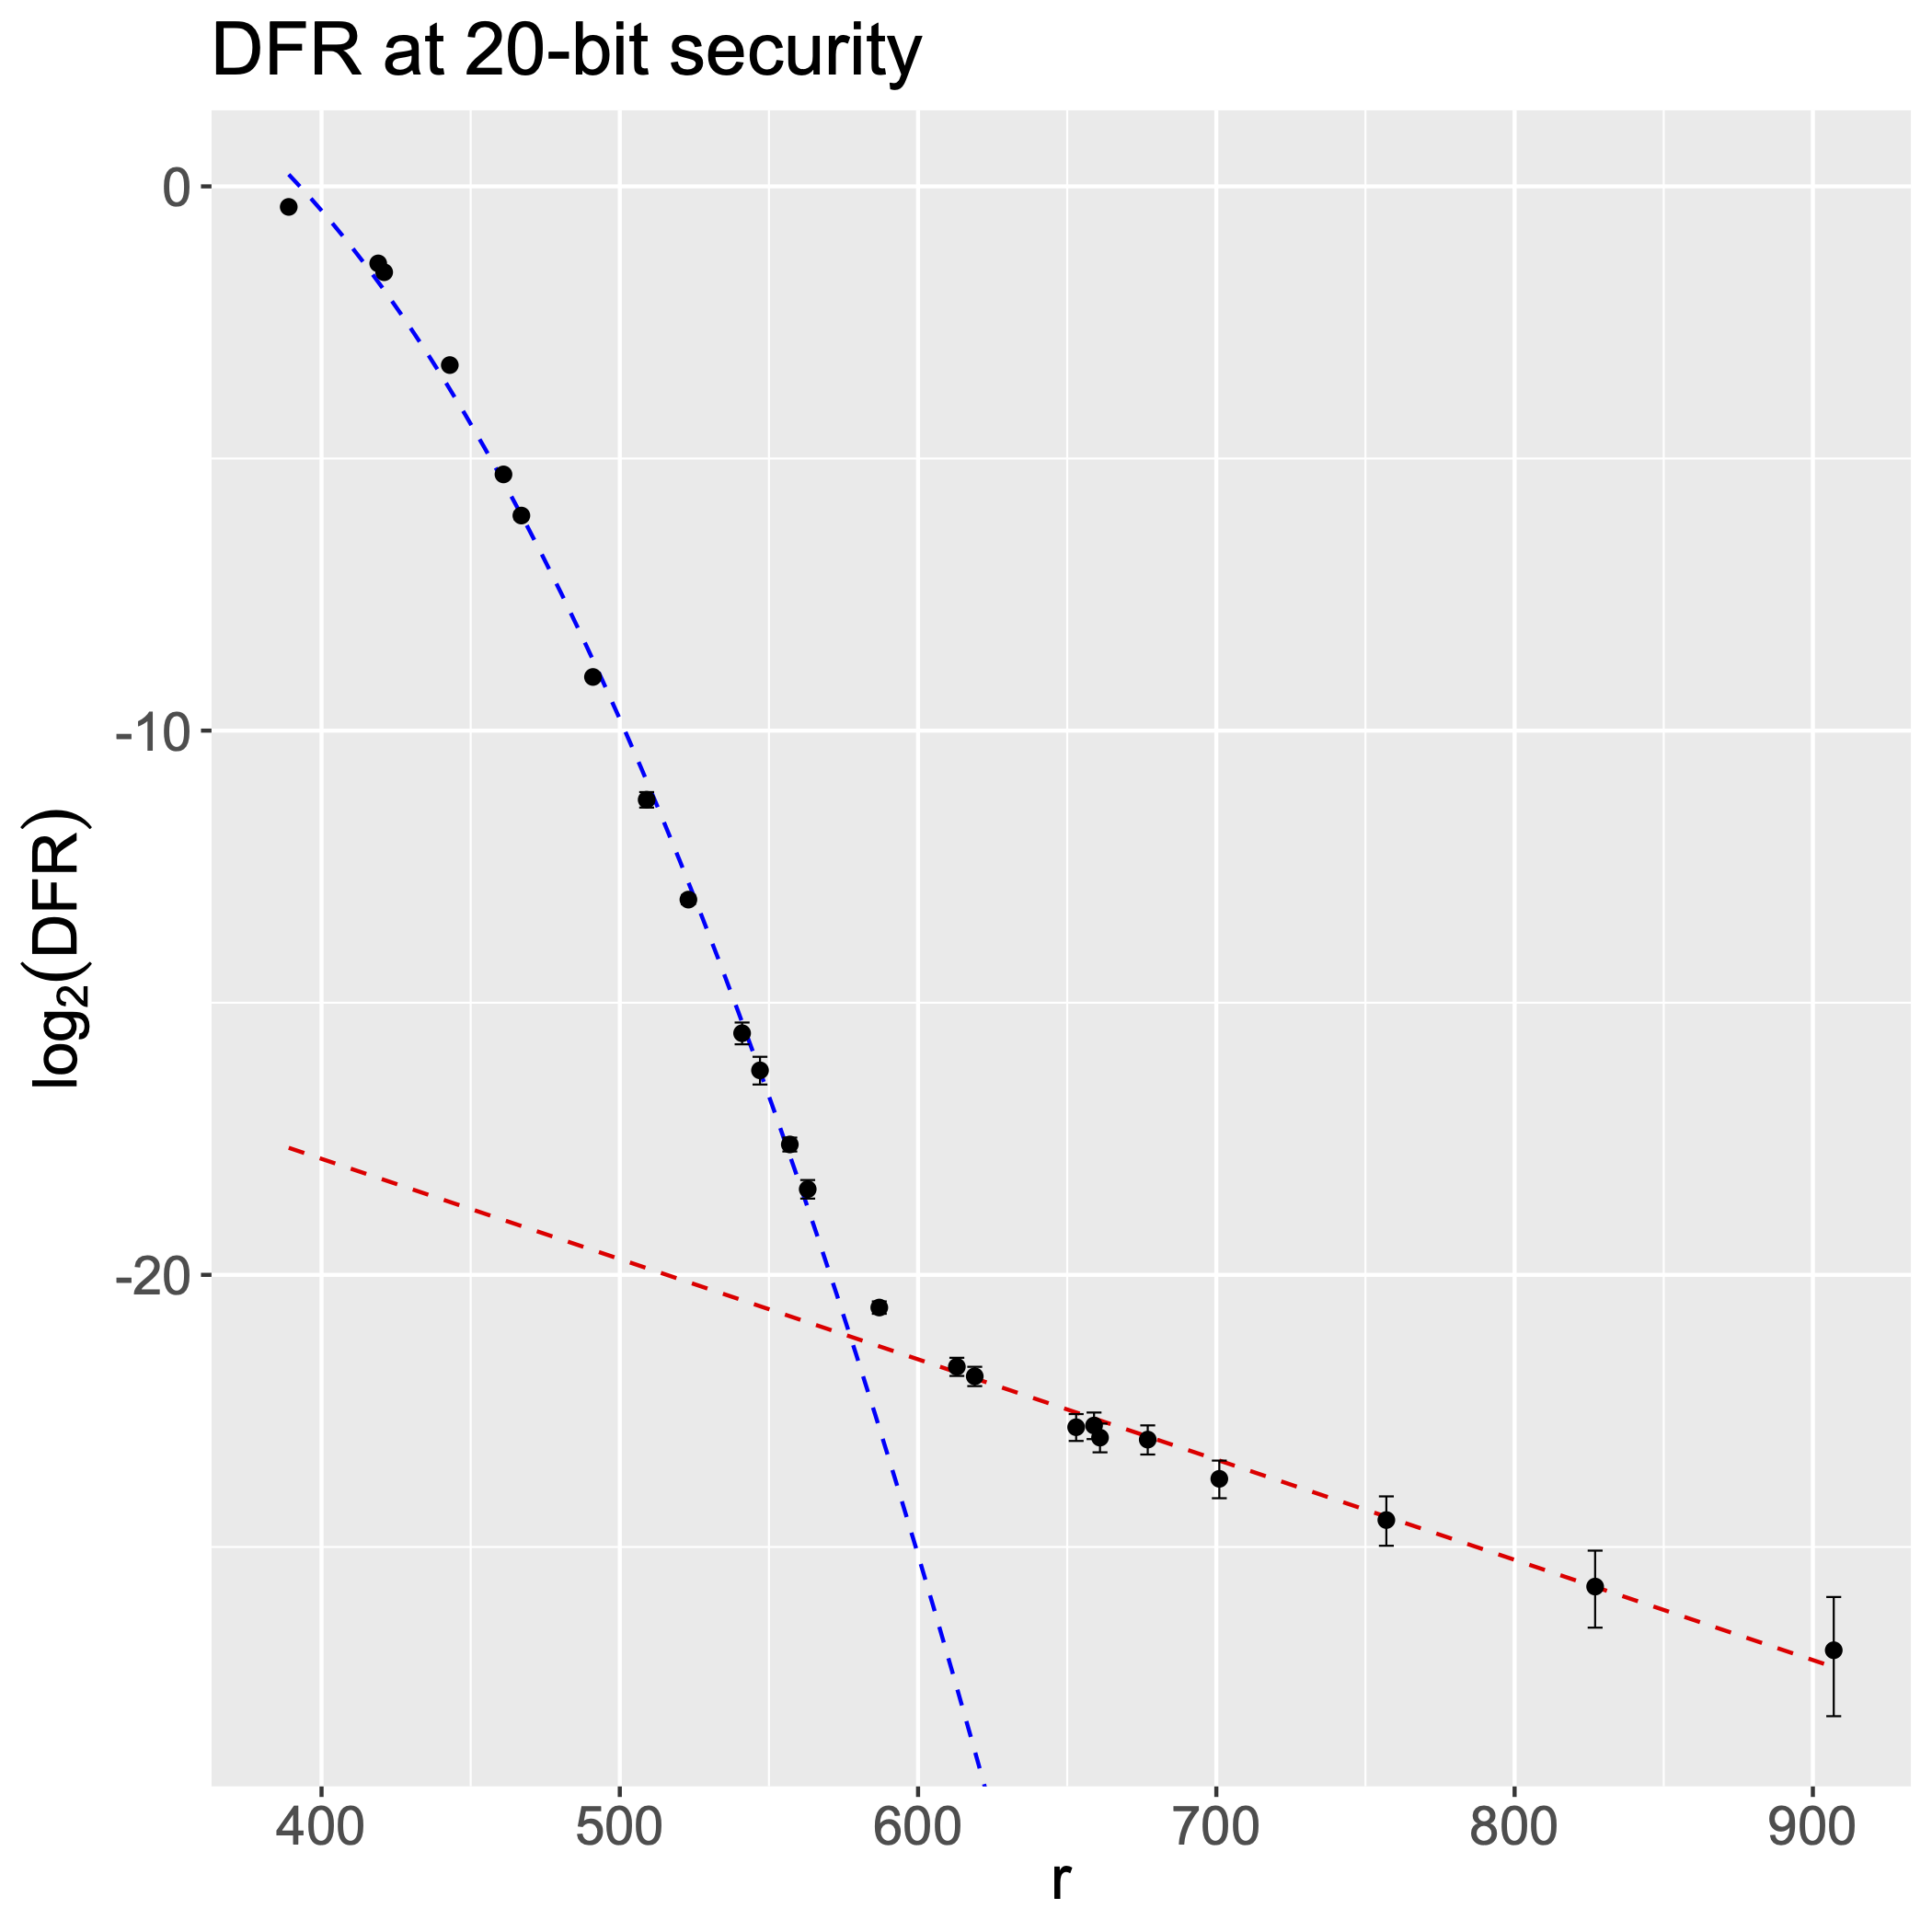
\includegraphics[scale=.07]{Images/DFR-plot-T3.png}
\end{figure}

\end{columns}
    
\end{frame}

\begin{frame}{Problematic error vectors}
In syndrome decoding, one issue can arise:

\begin{block}{Problem}
Given $H,s$, we may get $e_1$,$e_2$ such that:
     \[  He_1^T = s = He_2^T \iff e_1- e_2 \in C\]

    
\end{block}
Richardson considered \textbf{$(u,v)$ near-codewords}: error vectors $|e| = u$ such that $|He^T| = v$. 
    
    \begin{itemize}
        \item With $u,v$ small relative to $n$, the decoder might be trapped and return $|x| \leq t$ but $Hx^T = s$.
    \end{itemize}
    

\end{frame}


\begin{frame}{Problematic error vectors}

    Following Richardson, Vasseur identified $3$ problematic sets of error vectors:

    \begin{itemize}
        \item $\mathcal{C}$: the set of weight $w$ codewords;
        \item $\mathcal{N}$: the set of half rows of $H$;
        \item $2\mathcal{N}$: the set of sum of two elements of $\mathcal{N}$.
    \end{itemize}
    
    Idea:
    \begin{itemize}
        \item Correspond to Richardson's low weight codewords and $(u,v)$ near-codewords.
        \item Vectors close to $\mathcal{S}$ are more likely to be indistinguishable in the syndrome decoding problem.
    \end{itemize}

    
\end{frame}

\begin{frame}{Problematic error vectors}
        For $\mathcal{S} \in \{ \mathcal{C},\mathcal{N}, 2\mathcal{N}\}$, Vasseur defines:
    
    \[
    \mathcal{A}_{t,\ell}(\mathcal{S}) = \bigcup_{v \in \mathcal{S}} \{ e \in \FF_2^n| |e| = t, |e \star v| = \ell \}.
    \]
    
    If $e \in \mathcal{A}_{t,\ell}(\mathcal{S})$, there exists $v\in \mathcal{S}$ such that $|e \star v| = \ell$. We define the distance $\delta:= |v| + t - 2\ell$.
    
\end{frame}



\begin{frame}{DFR for special sets}
    For $r = 523,587,659$, we computed DFR on $\mathcal{A}_{18,\ell}(\mathcal{S})$ for various $\delta$.
    
    \begin{block}{Question}
    How does the DFR of $t \in \mathcal{A}_{18,\ell}(\mathcal{S})$ compare to the DFR of generic vectors $|e| = 18$ ?
    \end{block}
\end{frame}

\begin{frame}{DFR for special sets}
    \begin{figure}
    \centering
    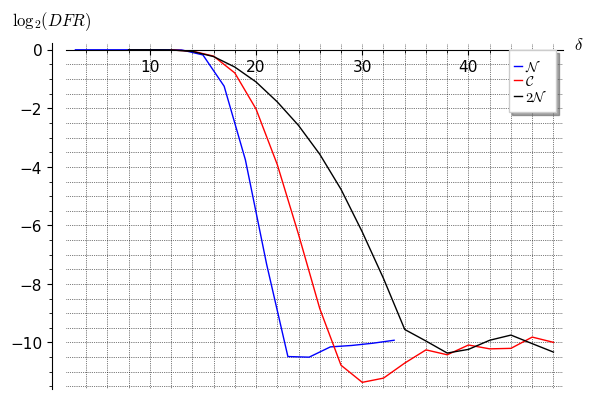
\includegraphics[scale=.6]{Images/DFR_20bit_CN2N_new.png}
    \caption{DFR vs $\delta$ for $r=587$}
\end{figure}

\end{frame}

\begin{frame}{Problematic vs generic error vectors}
    
    In our experiments, we recorded decoding failures. 
    
    \begin{block}{Question}
    How many overlaps do decoding failure vectors have with $\mathcal{C},\mathcal{N}, 2\mathcal{N}$?
    \end{block}
    
    For $r = 587$, we found the maximum number of overlaps with $\mathcal{S} \in \{\mathcal{C},\mathcal{N}, 2\mathcal{N} \} $ for each decoding failure vector. We repeat the experiment with random vectors and compare. 
    
\end{frame}


\begin{frame}{Problematic vs generic error vectors - data.}
\begin{columns}
    \column{0.5 \textwidth}
    \begin{figure}
    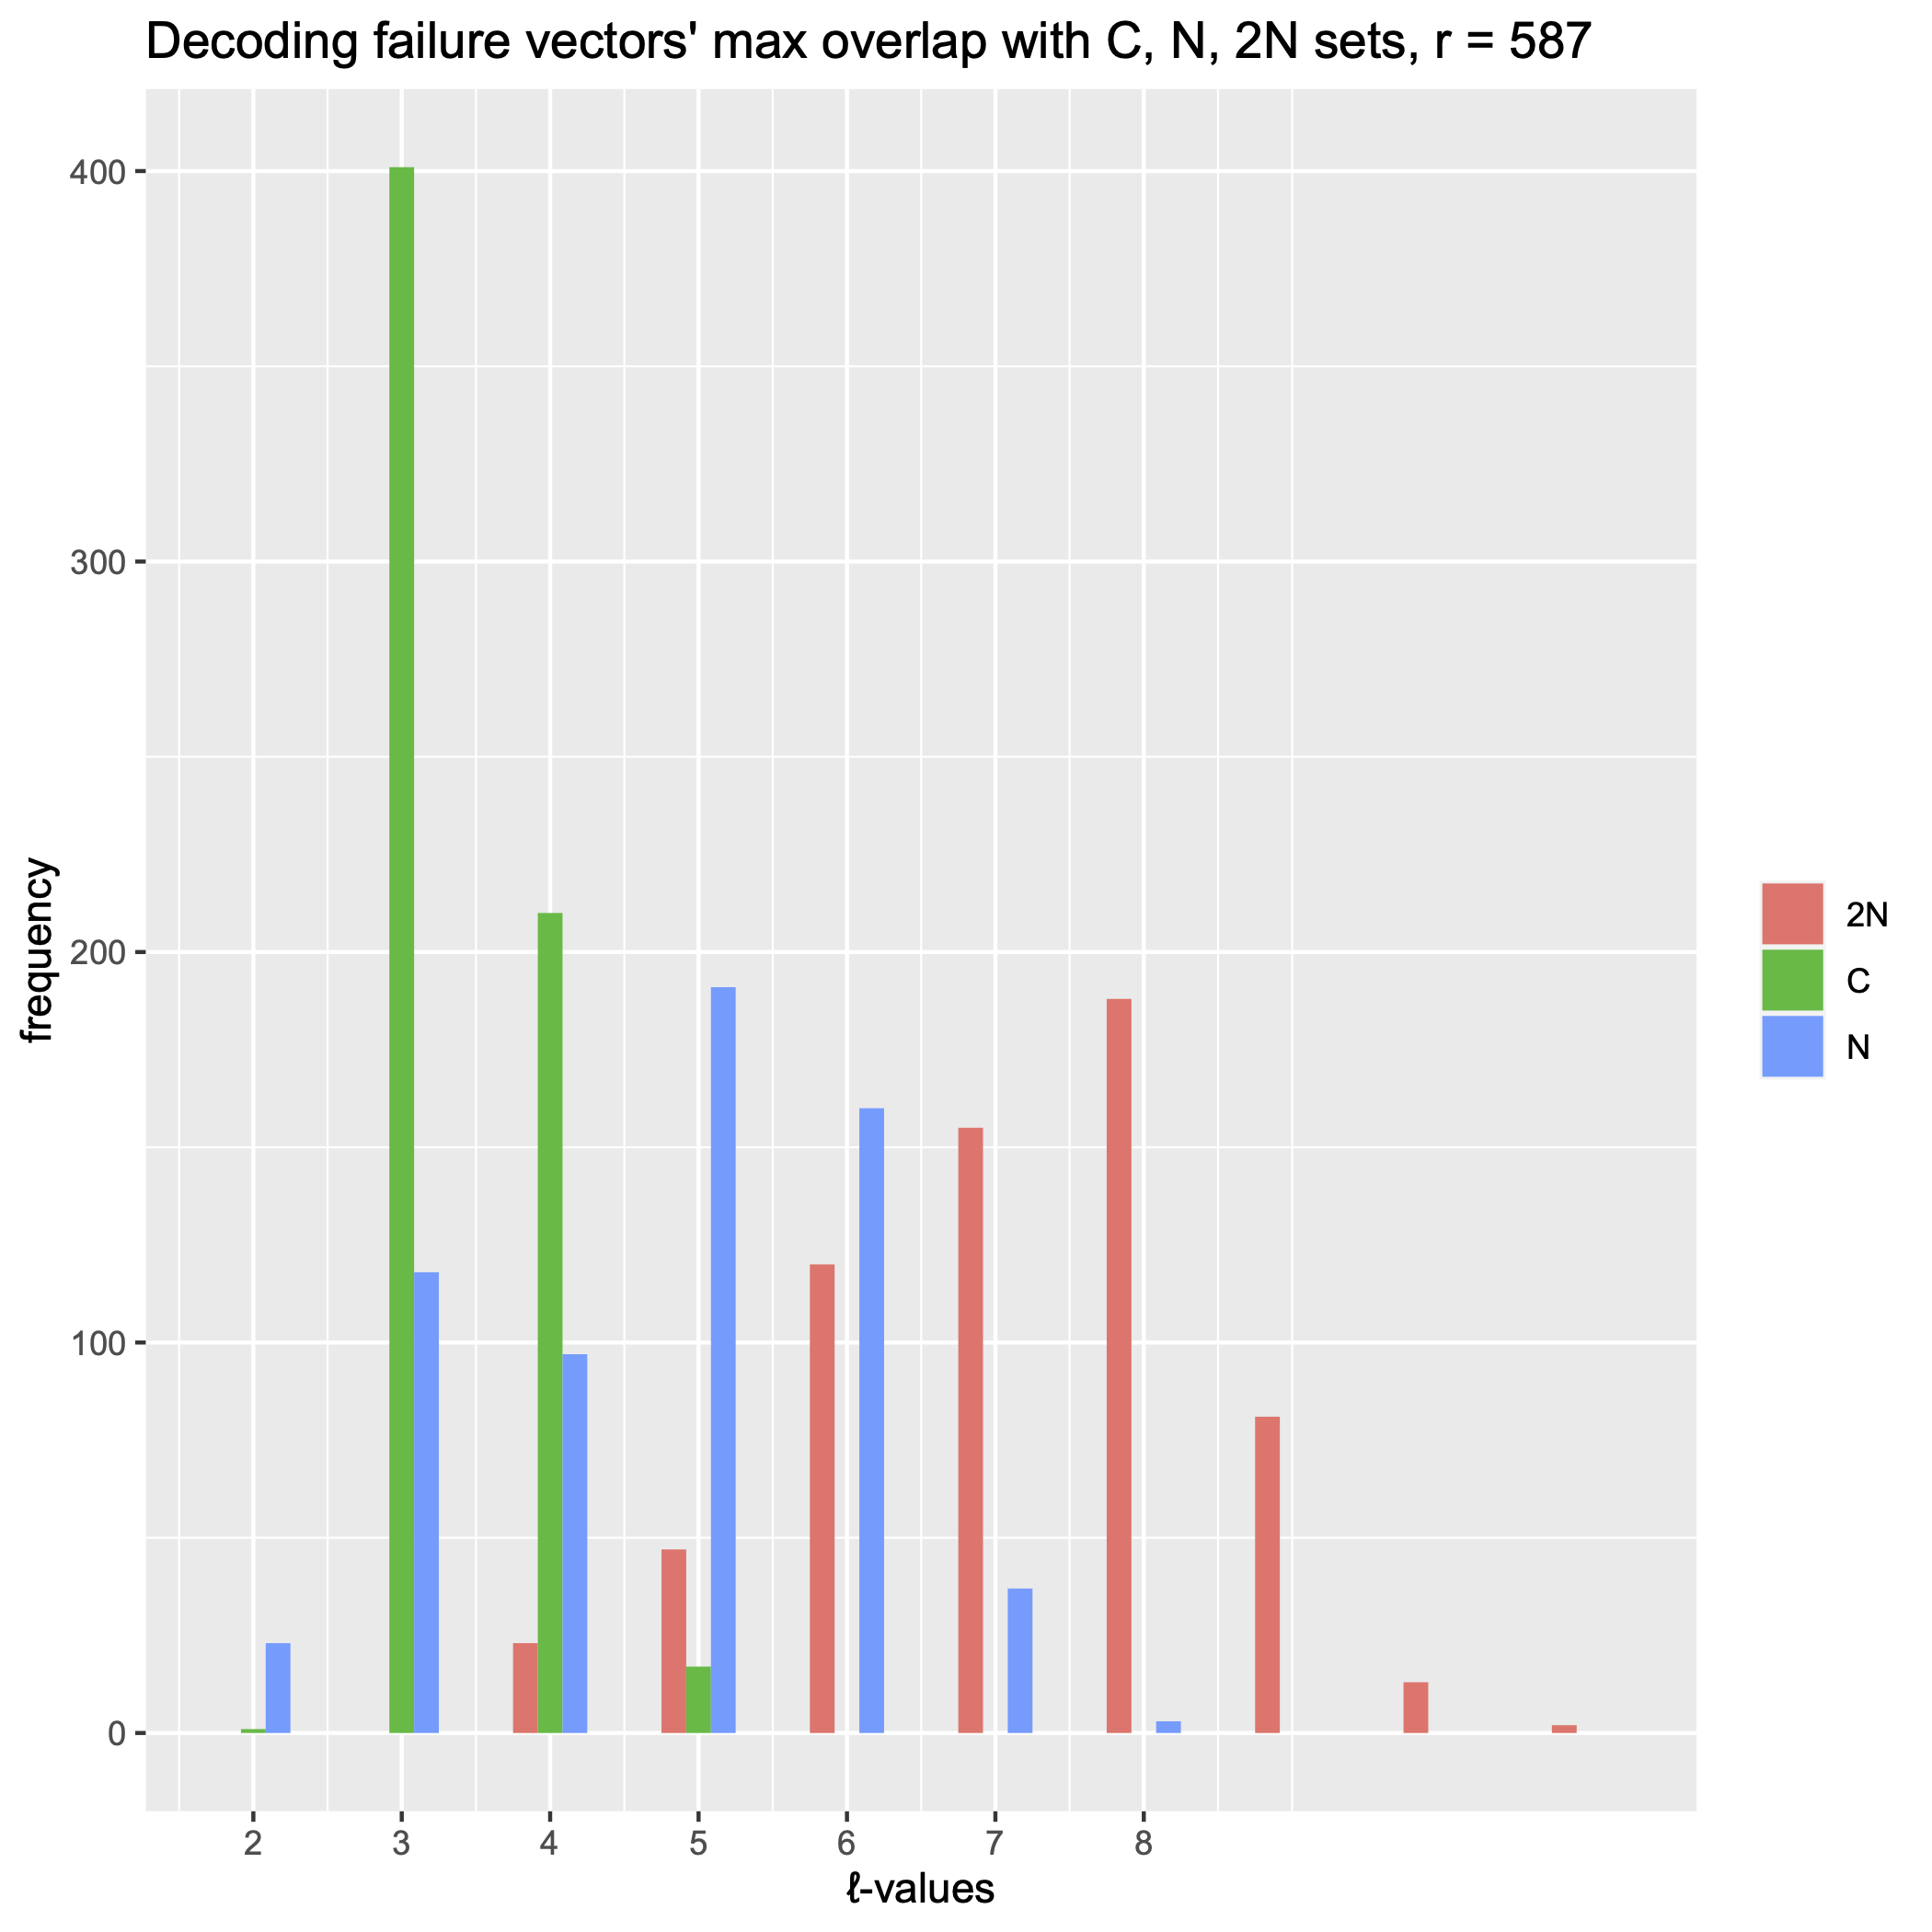
\includegraphics[scale=.06]{Images/Rplot-587-df.png}
    \caption{Decoding failure vectors}
    \end{figure}
    
    \column{0.5 \textwidth}
    \begin{figure}
    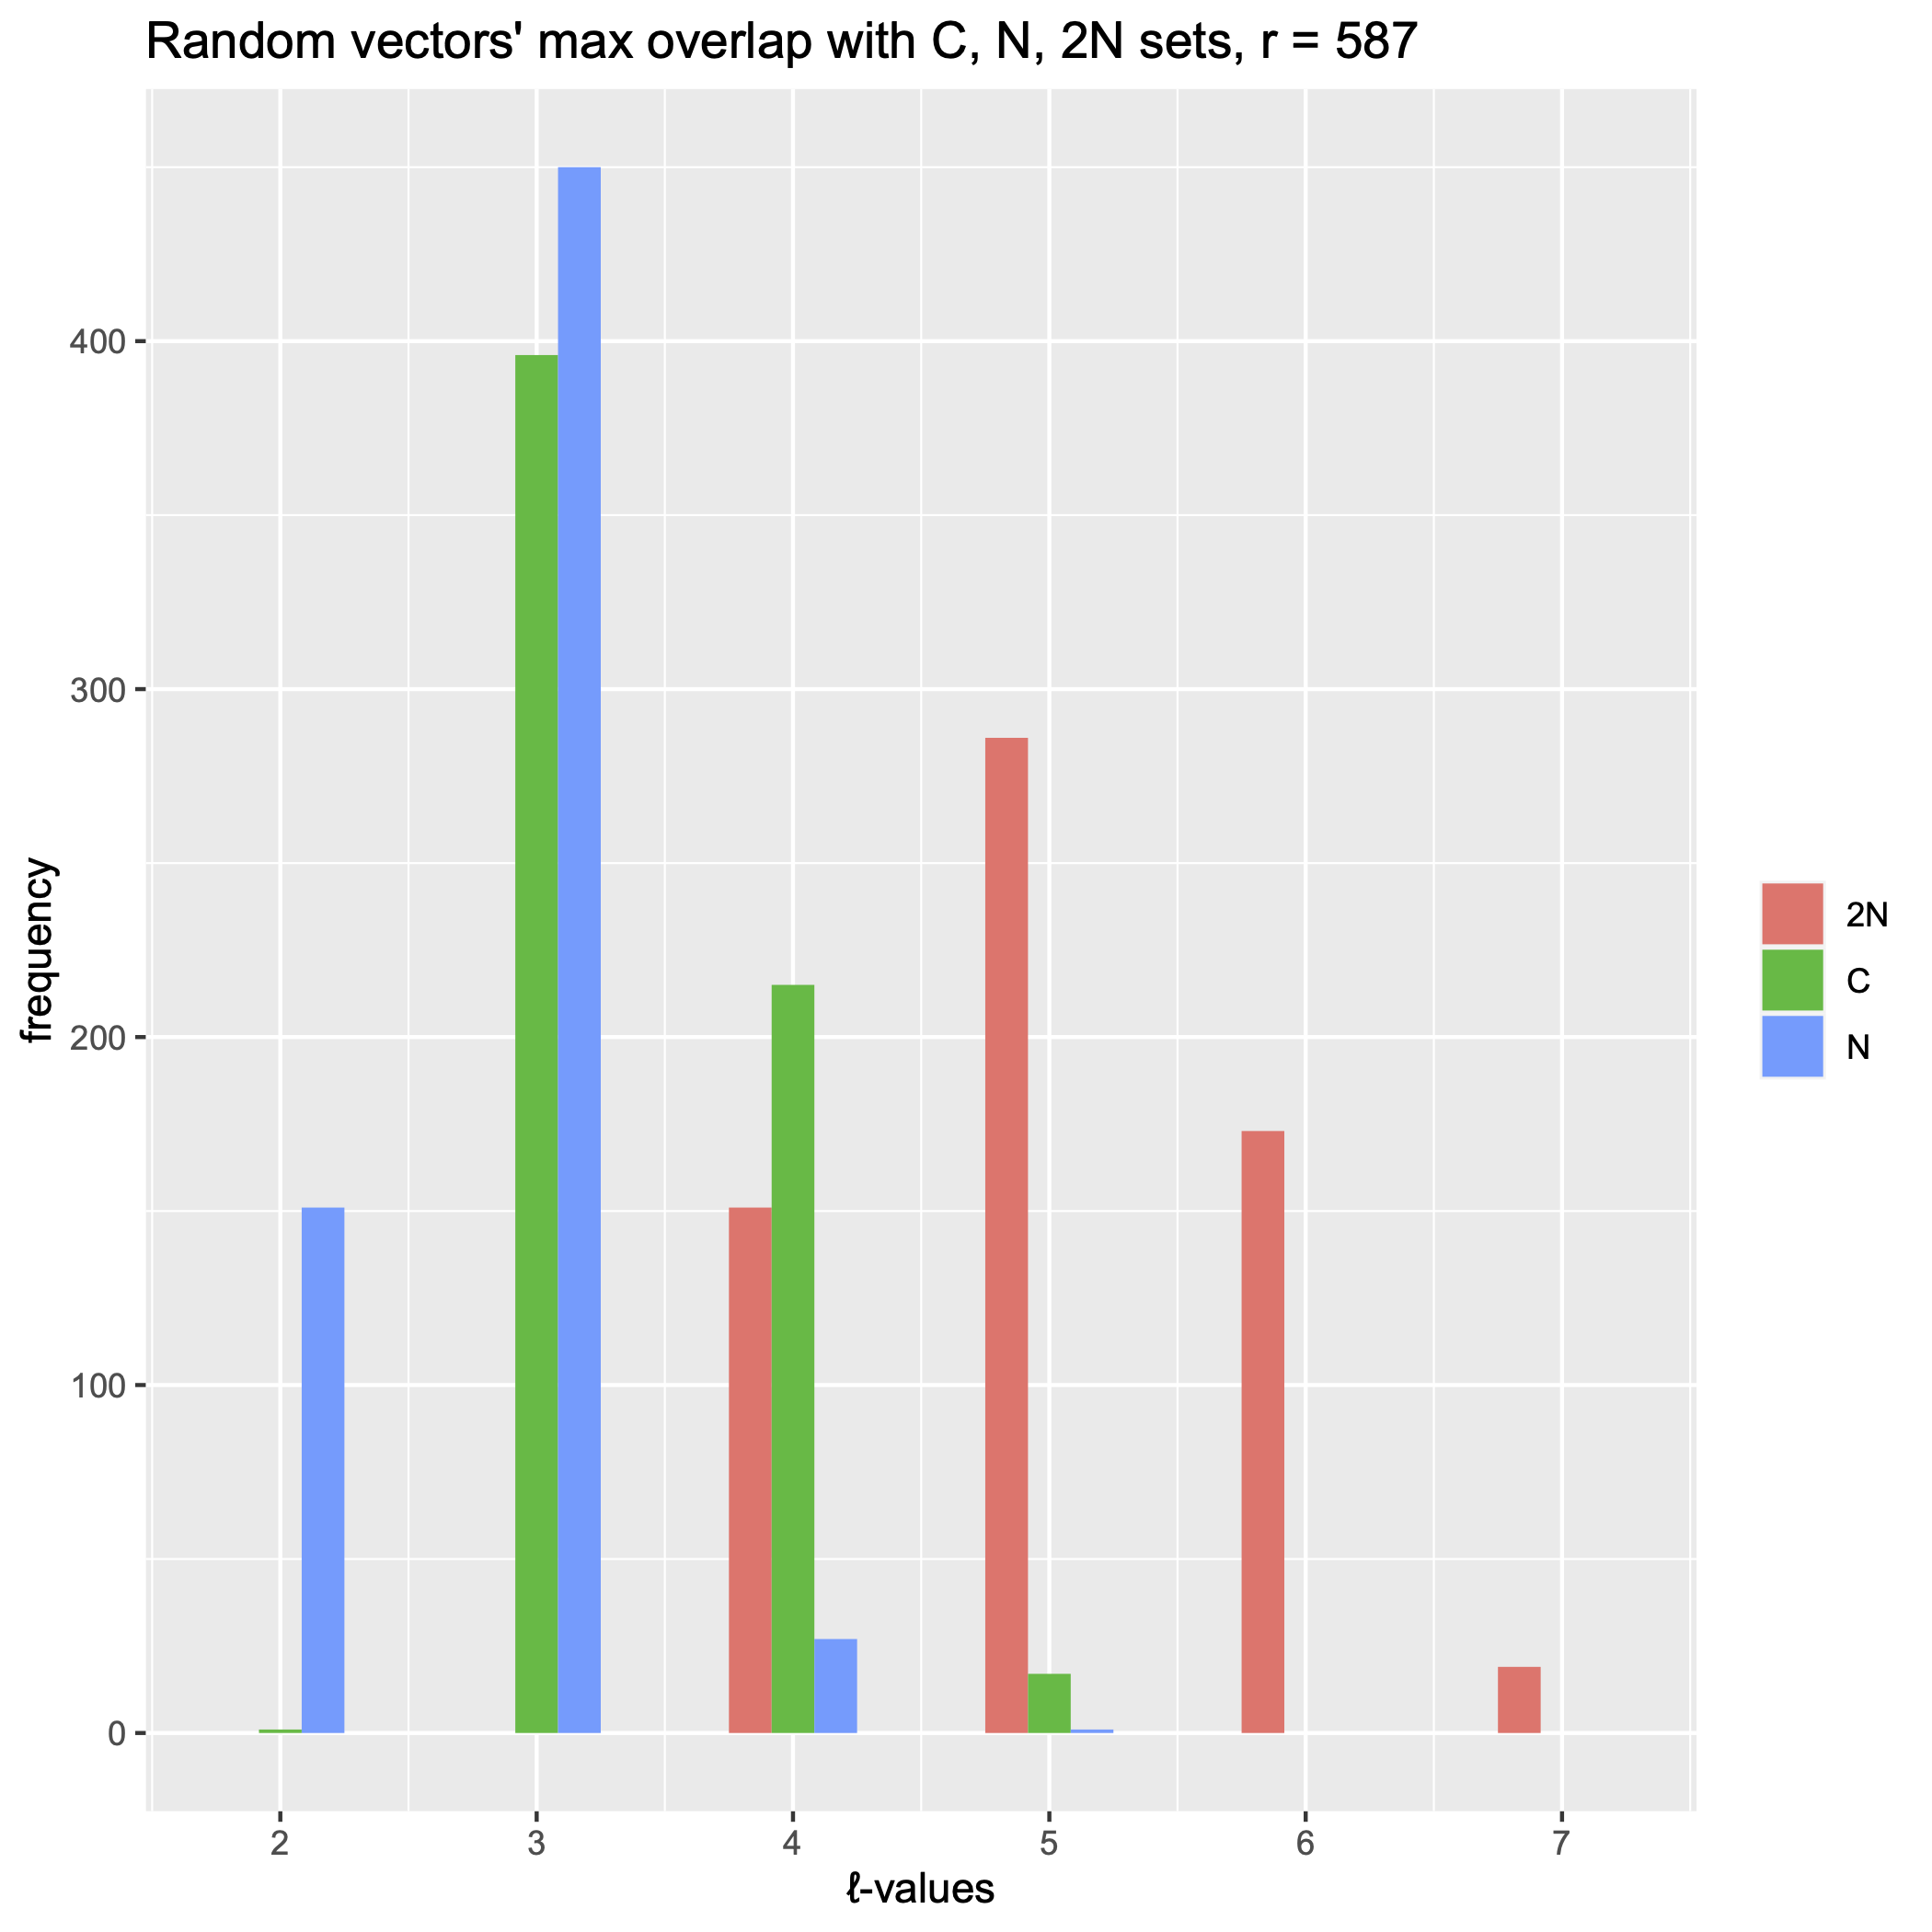
\includegraphics[scale=.06]{Images/Rplot-587-random.png}
    \caption{Randomly generated vectors}
    \end{figure}
\end{columns}

\begin{itemize}
\item Some proportion of decoding failures can be attributed to $\mathcal{N}, 2\mathcal{N}$.
\item A significant proportion of decoding failures do not have more overlap than typical random vectors.
\end{itemize}
\end{frame}

\begin{frame}{Syndrome weights of decoding failure vectors}
    From the DFR experiments of $\mathcal{A}_{t,\ell}(\mathcal{S})$, we observed that syndrome weights is an indicator of decoding failure.
    
    \begin{figure}
        \centering
        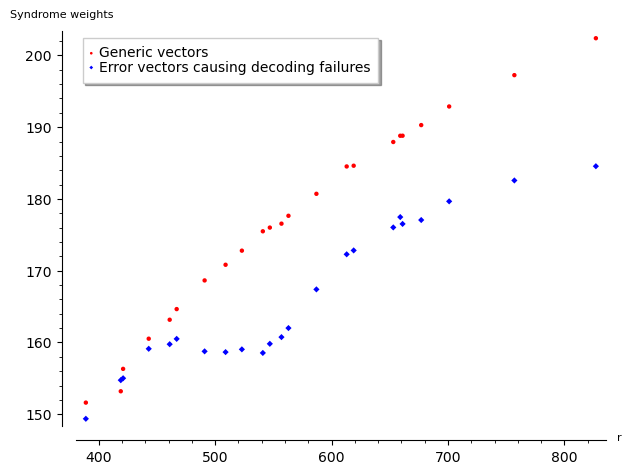
\includegraphics[scale=0.6]{Images/average_sw_generic_vs_DF_T3.png}
    \end{figure}
\end{frame}

\begin{frame}{Ongoing work}
    \begin{itemize}
        \item Apply graph theoretic techniques to study Tanner graphs of QC-MDPC codes.
\item Decoder behaviour (e.g., trapping sets, absorbing sets, etc.)
\item Syndrome weight and error floor phenomenon
    \end{itemize}
\end{frame}


\begin{frame}{}
    \centering
    Thank you!
  \end{frame}


\end{document}